\section{Raíces de Ecuaciones}
El problema de determinación de raíces (o de los ceros) de una función se 
presenta frecuentemente en diferentes aplicaciones de ingeniería y física. Acá 
discutiremos 2 métodos que pueden considerarse clásicos, como son el método de 
bisección y el método de Newton-Raphson. El primero tiene valor ya que es 
bastante intuitivo aunque no siempre eficaz, mientras que el segundo, al 
desprenderse de la expansión de una función en su serie de Taylor permite 
generalizarse a problemas de sistemas de ecuaciones.

\subsection{Planteamiento del problema}

Consideremos una función escrita de la forma
\begin{equation}
y=f(x)
\label{funcionY}
\end{equation}

la cual seguramente sabemos interpretar como una regla que transforma valores
de la variable independiente $x$ en valores de la variable dependiente $y$ y
donde $f(x)$ es la regla de la transformación, ver \cref{fig:ecuacion}.

\begin{figure}[H]
	\centering
	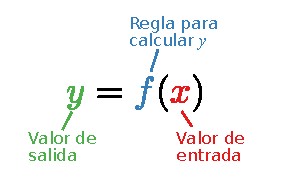
\includegraphics[width=50 mm]{ecuacion.pdf}
	\caption{Descripción del concepto de función como una regla de
	transformación de valores (posiblemente) reales  en otros valores
	(posiblemente) reales.}
	\label{fig:ecuacion}
\end{figure}

Por ejemplo, un caso particular de una regla de transformación o función puede 
ser de la forma:
\[f(x) = \ x^3 + 4x^2 - 10\, .\]

El problema de búsqueda de raíces de la función consiste en encontrar valores 
de la variable independiente $x$ que cuando sean transformados por la regla 
$f(x)$ produzcan valores nulos de $y$. Matemáticamente esta pregunta la podemos 
plantear como encontrar valores de $x$ que satisfagan la condición:
\[f(x) = 0.0\, .\]

Por ejemplo, la \cref{fig:raiz} muestra la variación de la función
\[f(x) = \ x^3 + 4x^2 - 10\, ,\]
para valores de $x$ en el intervalo $[-4, 2].$ En la gráfica el círculo blanco 
correspondiente a la intersección de la línea $y=0$ y la función corresponde a 
una raíz de la función. Esta tiene un valor aproximado de $x=1.4.$

\begin{figure}[H]
	\centering
	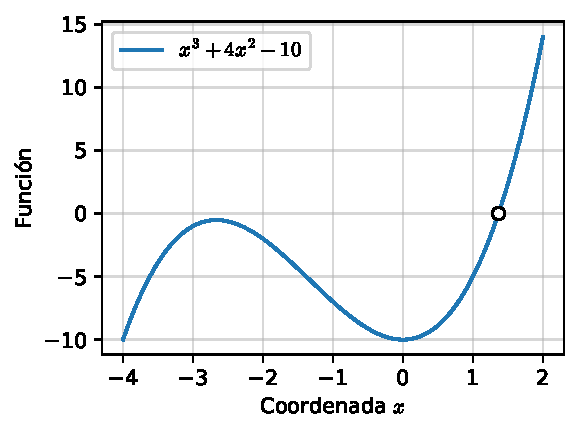
\includegraphics[width=4 in]{raiz.pdf}
	\caption{Concepto de raíz de una función. La función sobre el intervalo
	$[-4.0, 2.0]$ se muestra con la línea azul y la raíz con el círculo blanco.}
	\label{fig:raiz}
\end{figure}


La función puede tener varias raíces reales (positivas o negativas) o inclusive
varias raíces complejas.

\paragraph{Ejemplo: Determinación de caudal.}
Un problema típico en ingeniería hidráulica es el de determinar el caudal $Q$ 
con el que es necesario alimentar una turbo-máquina de potencia especifica
$\phi$, resistencia total a fluir $R_T$ la cual está localizada entre 2 niveles 
con salto $\Delta H$. Usando argumentos de conservación de energía se puede 
demostrar que este caudal satisface la condición:

\begin{equation}
	{R_T}{Q^3} - \Delta HQ + \phi  = 0.
\label{caudal}
\end{equation}

Claramente, se trata de un problema de determinación de raíces tras encontrar 
el caudal $Q$ que satisfaga la condición:
\[f(Q) = 0.0\, ,\]
donde
\begin{equation}
f(Q) ={R_T}{Q^3} - \Delta HQ + \phi\, .
\label{caudalF}
\end{equation}

\begin{tcolorbox}
En computación se denomina \textbf{iteración} un procedimiento que se aplica al 
resultado de una operación previa.
\end{tcolorbox}

En general, los métodos de determinación de raíces son iterativos y requieren 
de una estimación inicial de la raíz (o raíces). De acuerdo con dicha 
estimación se pueden tener los siguientes resultados (ver 
\cref{fig:raizconverge}):
\begin{itemize}
	\item Falla de convergencia.
	\item Convergencia a un valor incorrecto.
	\item Convergencia a un valor correcto.
\end{itemize}

Antes de iniciar el estudio de un par de métodos clásicos para 
determinación de raíces es importante tener una idea de los conceptos de 
convergencia y divergencia. Intuitivamente, decimos que un método converge 
cuando los valores se acercan cada vez más y que diverge cuando pasa lo 
contrario, se alejan entre ellos. Adicionalmente, llamamos \textbf{tasa de 
convergencia} a la rapidez con la que un cálculo iterativo se aproxima a una 
solución. Ahora, concentrémonos en la \cref{fig:raizconverge} en la cual se 
grafica la variación del error vs el número de iteraciones en un algoritmo. 
La gráfica presenta el porcentaje de error contra el número de iteraciones 
requeridas para predecir la raíz $x=1.3652305$ por medio de los 2 métodos que 
estudiaremos en esta sección a saber el método de bisección y el método de 
Newton. Podemos ver que uno de los métodos converge más rápidamente que el otro.

\begin{figure}[H]
  \centering
  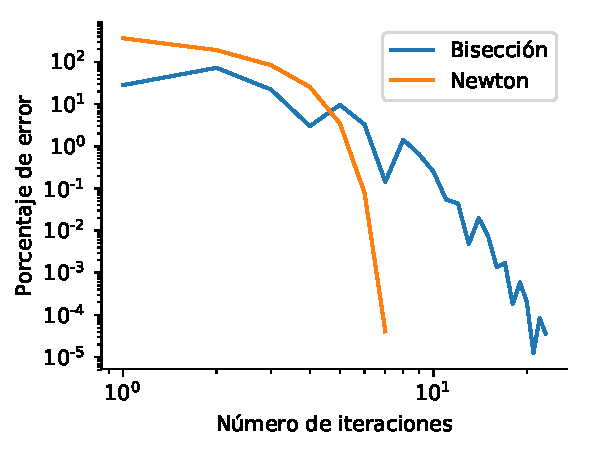
\includegraphics[width=4 in]{convergencia.pdf}
  \caption{Concepto de convergencia o número de iteraciones requeridas para
  alcanzar una solución.}
  \label{fig:raizconverge}
\end{figure}
	

\subsection{Localización incremental de raíces}

El cálculo de las raíces de una ecuación involucra 2 procesos que se discutirán 
a continuación. Inicialmente se identifican de manera aproximada las 
localizaciones de las raíces en un intervalo determinado. Este proceso se 
denomina \textbf{detección} o \textbf{bracketing}. El proceso de detección 
arroja valores de las raíces con baja precisión.

Para mejorar la precisión se ejecuta un segundo paso tras seleccionar una 
precisión especificada mediante una \textbf{tolerancia} o valor de referencia. 
La tolerancia indica cual es la definición aceptable de cero para determinar si 
efectivamente se encontró la raíz. Esta es necesaria ya que en el computador 
solo es posible especificar el cero hasta cierto número de cifras 
significativas, en otras palabras, en el computador no existe el cero 
matemático. El segundo proceso corresponde entonces al acercamiento a la raíz 
con una precisión dada y definida en términos de la tolerancia. Este segundo 
paso se denomina \textbf{determinación} de la raíz. En resumen, el 
proceso de búsqueda de raíces implica 2 pasos:

\begin{itemize}
	\item[i.] Localización inicial de las raíces o {\bf Detección}.
	\item[ii.] Acercamiento o mejoramiento en la precisión del valor de la
	raíz o {\bf Determinación}.
\end{itemize}

En el proceso de detección de la raíz la idea fundamental consiste en recorrer 
la función por intervalos de tamaño $\Delta x$ y con límites $x_1$ y $x_2$. Si 
durante el recorrido se encuentra que los valores $f(x_1)$ y $f(x_2)$ de las 
funciones tienen signos diferentes, entonces se concluye que existe al menos 
una raíz en el intervalo. El proceso se resume en los siguientes 2 pasos:

\begin{itemize}
	\item[i]  Recorrido del dominio por intervalos $\Delta x$.
	\item[ii] Evaluación de la función para detectar cambios de signo.
\end{itemize}

Para explicar el proceso y su eventual solución en el computador tomemos como 
referencia la \cref{fig:bracketing} en la que se presenta una función que tiene 
2 raíces (círculos negros) en el intervalo $[a,b]$. El proceso de detección se 
describe además en el \cref{alg:brack}. Los datos de entrada al problema son 
los extremos del intervalo correspondientes a $x=a$ y $x=b$; el número de 
subintervalos $N$ en los que se partirá el dominio del problema; y la función 
$f(x)$ cuya raíz se desea determinar.  El algoritmo entregará como resultado 
las raíces encontradas, las cuales almacenará en un vector denominado $x_R$. En 
el primer paso del algoritmo calculamos el tamaño del subintervalo $\Delta x$ y 
fijamos el contador de detección de raíces $iroot$ en cero. Este contador se 
incrementará en 1 cada que el algoritmo detecte una raíz.

La parte principal del algoritmo consiste en un ciclo que recorre los $N$ 
subintervalos en los que se ha partido el problema y detecta cambios de signo 
haciendo evaluaciones del producto $f (x_1) \times f (x_2).$ Si se da la 
condición $f \left( x_1 \right) \times f \left( x_2 \right) < 0.0$ entonces se 
concluye que existe una raíz en algún punto entre $x=x_1$ y $x=x_1+ \Delta x$. 
Este evento queda registrado en el contador $iroot$. Al mismo tiempo se 
selecciona el inicio del intervalo como el de localización aproximada de la 
raíz. Esta se almacena en la posición $irrot$ del vector $x_R$ . Este algoritmo 
sencillo se da como referencia en el apéndice de estas notas.

\begin{figure}[H]
\centering
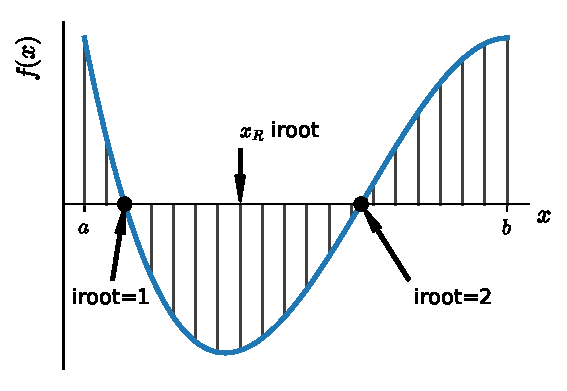
\includegraphics[width=4 in]{busquedas_inc.pdf}
\caption{Proceso de detección de raíces de una función en un intervalo $[a,b]$.}
\label{fig:bracketing}
\end{figure}


\begin{algorithm}[H]
\SetAlgoLined
\KwData{$a, \ b, \ N, \ f$}
\KwResult{$x_R$: Vector con la aproximación de las raíces}
\BlankLine

$\Delta x \leftarrow \dfrac{b - a}{N - 1}$;\\
\BlankLine
$iroot \leftarrow 0$ ;\\
\BlankLine
$x_2 \leftarrow a$ ;\\
\BlankLine
\For{$i \leftarrow 0$ to $N - 1$}{
	$x_1 \leftarrow x_2$;\\
	$x_2 \leftarrow x_1+\Delta x$;\\
	\If{$f (x_1) \times f (x_2) <0.0$}{
		$iroot \leftarrow iroot+1$;\\
		$x_R [i] \leftarrow x_1$;\\
		}
	\BlankLine
	}
\BlankLine
\caption{Detección o \textit{bracketing}.}
\label{alg:brack}
%
\end{algorithm}

La aplicación del código anterior a la función $f(x) = \ x^3 + 4x^2 - 10$ en el 
intervalo comprendido entre $a=-10.0$ y $b=10.0$ con $\Delta x = 1.0$ produce 
el vector de raíces $x_R$
\begin{verbatim}
A change of sign was found.
[0. 0. 0. 0. 0. 0. 0. 0. 0. 0. 0. 1. 0. 0. 0. 0. 0. 0. 0. 0. 0.]
\end{verbatim}
el cual indica que la función tiene un cero en el intervalo $[1.0,2.0]$ y 
localizado aproximadamente en $x = 1.0$. Este valor de la raíz debe ser 
posteriormente refinado para encontrar el valor consistente con la tolerancia 
prescrita. En las secciones que se presentan a continuación discutiremos 2 
métodos clásicos usados para realizar este refinamiento de la raíz.


\subsection{Método de bisección}
En este paso se asume que ya se ha encerrado una raíz de $f(x) = \ 0.0$ en el intervalo $(x_1, x_2)$ mediante un proceso previo de detección.  Tal y como se describe en la \cref{fig:bisection}, la raíz se encuentra en algún punto entre $x_1$ y $x_2$. Mas aún, el algoritmo de detección entrega como localización aproximada de la raíz $x = x_1$. El siguiente paso consiste entonces en acercarse a la raíz con una precisión deseada. El método de bisección consiste en la partición por mitades del intervalo $\Delta x$ en el que se encuentra localizada la raíz alternando entre posiciones de cambio de signo. Cada que se detecta el cambio de signo se redefine el intervalo de la raíz y esta partición continúa hasta que el intervalo se haga lo suficientemente pequeño. El algoritmo localiza inicialmente el punto intermedio ${x_3} = \frac{1}{2}(x_1 + x_2)$ ubicado entre los extremos del intervalo $x_1$ y $x_2$.

\begin{figure}[H]
\centering
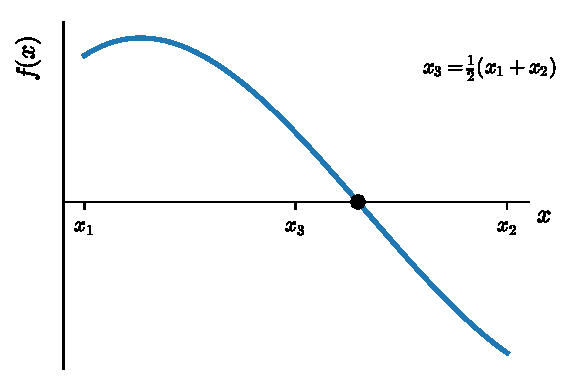
\includegraphics[width=4 in]{biseccion.pdf}
\caption{Método de bisección para encontrar las raíces.}
\label{fig:bisection}
\end{figure}

Si $f (x_1) \times f (x_3) < 0.0 $ entonces existe una raíz entre $x_1$ y $x_3$ en cuyo caso se hace $x_2	\leftarrow x_3$ y se calcula un nuevo ${x_3} = \frac{1}{2}({x_1} + {x_2})$ dividiendo a la mitad el intervalo que contiene a la raíz. Si por el contrario se determina que $f (x_1) \times f (x_3) > 0.0 $ entonces la raíz se localiza entre $x_3$ y $x_2$ en cuyo caso se hace $x_1	\leftarrow x_3$ y se calcula un nuevo ${x_3} = \frac{1}{2}({x_1} + {x_2})$ dividiendo nuevamente el intervalo. Este proceso se resume en la siguiente tabla.
\begin{table}[H]
  \centering
  \begin{tabular}{ll}
	Si $f (x_1) \times f (x_3) < 0.0 $\\ & Raíz entre $x_1$ y $x_3$\\ 
	  & $x_2	\leftarrow x_3$ \\
	  & $x_3 \leftarrow \dfrac{1}{2} (x_1 + x_2)$ \\
	  & Calcula $\Delta x \leftarrow x_3-x_1$ \\\\
	Si $f (x_1) \times f (x_3) > 0.0 $\\ & Raíz entre $x_3$ y $x_2$\\ 
      & $x_1	\leftarrow x_3$ \\
      & $x_3 \leftarrow \dfrac{1}{2} (x_1 + x_2)$ \\
      & Calcula $\Delta x \leftarrow x_2-x_3$
  \end{tabular}
\end{table}

El \cref{alg:repeat} presenta el pseudocódigo para el método de bisección.
\begin{algorithm}[h]
\SetAlgoLined
\KwData{$a, \ b, \ tol, \ f$}
\KwResult{$c$: Aproximación de la raíz}
Set $tol$;\\
$n_{\max}  \leftarrow \ceil{\log_2\left(\frac{b - a}{tol}\right)}$ ;\\
\For{cont $\leftarrow 0$ to $n_{\max}$}{
    $c \leftarrow  \frac{1}{2}(a + b)$;\\
	\eIf{$f (a) f (b) < 0.0$}{
		$b \leftarrow c$;\\
		}{
		$a \leftarrow c$;\\
		}
	\BlankLine
	}
\BlankLine
\caption{Bisección}
\label{alg:repeat}
\end{algorithm}

En el apéndice se presenta el código en Python correspondiente al algoritmo de 
bisección el cual arroja el siguiente resultado tras aplicarlo a la función $f 
(x) = \ x^3 + 4x^2 - 10$, sobre el intervalo [-2, 2], usando una tolerancia 
$tol = 10^{-4}$.

\begin{verbatim}
n: 0, x: 0.0
n: 1, x: 1.0
n: 2, x: 1.5
n: 3, x: 1.25
n: 4, x: 1.375
n: 5, x: 1.3125
n: 6, x: 1.34375
n: 7, x: 1.359375
n: 8, x: 1.3671875
n: 9, x: 1.36328125
n: 10, x: 1.365234375
n: 11, x: 1.3642578125
n: 12, x: 1.36474609375
n: 13, x: 1.36499023438
n: 14, x: 1.36511230469
n: 15, x: 1.36517333984
Maximum number of iterations reached.
1.36517333984375
\end{verbatim}

\subsection{Método de Newton-Raphson}

\textcolor{blue}{Este método tiene la desventaja de que requiere, además de la 
evaluación de la función $f(x)$, también la de su primera derivada $f'(x)$.}

El método de Newton-Raphson suele converger más rápido que el método de 
bisección. Esto se debe a que se incluye más información sobre la función en 
las iteraciones, a saber, las derivada. Por la forma que toma la iteración la 
función debe tener un valor diferente de cero para cada aproximación. Como se 
discutió anteriormente las iteraciones se detiene una vez se alcance el cero 
dentro de una tolerancia prescrita.

\subsubsection*{Derivación matemática}
Sea $x_i$ la $i$-ésima\footnote{Por ejemplo, $x_0$ es el valor 
encontrado por el algoritmo de detección.} aproximación a la raíz buscada y $p$ 
el valor refinado de la raíz que se encuentra en la vecindad de 
$x_i$. Escribiendo la función como una serie de Taylor alrededor de $p$ se 
tiene:
\[f(p)=f(x_i)+f'(x_i)(p-x_i)+{(p-x_i)}^2\frac{f''(x_i)}{2!}+...\]

Luego, asumiendo que $f(p)$ es cercano a cero ($f(p)\approx0$) y linealizando 
se tiene:
\[ 0\approx f(x_i)+f'(x_i)(p-x_i) \]
haciendo $x_{i+1}\equiv p$ y re-escribiendo se tiene la expresión
\[x_{i+1}\approx x_i-\frac{f(x_i)}{f'(x_i)}\]
correspondiente a la iteración de Newton-Raphson que permite determinar la raíz 
aproximada  $x_{i+1}$ a partir de la aproximación $x_i$.

\begin{tcolorbox}
Se denomina \textbf{linealización} a la operación de eliminar los términos de 
orden 2 y superiores y retener solo los términos lineales en una expresión. 
La iteración de Newton-Raphson corresponde a la serie de Taylor 
linealizada de la expansión de la función alrededor de la raíz buscada.
\end{tcolorbox}

\subsubsection*{Derivación geométrica}
Geométricamente, el método de Newton-Raphson consiste en extender la recta 
tangente en el punto actual $x_i$ hasta que cruce el cero para luego hacer la 
siguiente aproximación  en la abscisa de dicho punto de cruce. El proceso se 
ilustra en la \cref{fig:newton} en donde se ve que para iniciar las 
iteraciones se requiere una aproximación inicial ($x_0$) a la raíz. Este valor 
inicial es el encontrado mediante el algoritmo de detección discutido 
anteriormente.

Para derivar el método desde una mirada geométrica partiremos del punto $x_i$, 
encontraremos la recta tangente que pasa por el mismo y lo extenderemos hasta 
su cruce con cero, como ya se describió. Usando la ecuación de la pendiente, 
tenemos
\[m = \frac{0 - f(x_i)}{x_{i+1} - x_i}\, ,\]
pero, sabemos que la pendiente es $m = f'(x_i)$, luego
\[f'(x_i) = -\frac{f(x_i)}{x_{i + 1} - x_i}\, ,\]
y si resolvemos esta ecuación para $x_{i +1}$ obtenemos el punto para el cual 
la recta toma el valor de cero. Este será el nuevo punto inicial para repetir 
el proceso y correspondiente a la iteración de Newton-Raphson.
\begin{equation}
  x_{i + 1} = x_i - \frac{f(x_i)}{f'(x_i)}
  \label{eq:iteracion_newton}
\end{equation}

\begin{figure}[H]
\centering
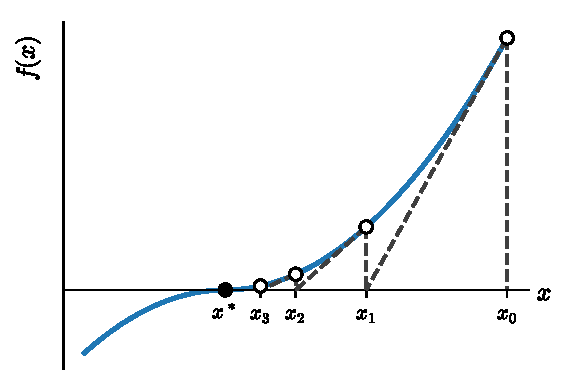
\includegraphics[width=4 in]{newton_iter.pdf}
\caption{Iteración de Newton-Raphson.}
\label{fig:newton}
\end{figure}


 El \cref{alg:newton} presenta el método de Newton para un punto inicial $x$ 
 mientras que su correspondiente código en Python se presenta en los apendices.

\begin{algorithm}[H]
\SetAlgoLined
\KwData{$x, \ tol, \ n_{\max}, \ f, \ f'$}
\KwResult{Raíz aproximada}
\For{cont $\leftarrow  0$ to $n_{\max}$}{
	\If{$|f'(x)| < tol$}{
		Error, división por número cercano a cero.\\
		}
    $x \leftarrow x - \frac{f(x)}{f'(x)}$;\\
	\If{$|f(x)| < tol$}{
		Pare, se llegó al valor deseado.
		}
	}
\BlankLine
\caption{Newton-Raphson}
\label{alg:newton}
\end{algorithm}



Si se aplica el código correspondiente al algoritmo anterior a la función $f (x) = \ x^3 + 4x^2 - 10$ usando una tolerancia $tol = 10^{-8}$ y una estimación inicial de la raíz correspondiente a $x_2=2.0$ de acuerdo al resultado del algoritmo de detección se obtiene el siguiente resultado tras 4 iteraciones.
\begin{verbatim}
n: 0, x: 2.0
n: 1, x: 1.5
n: 2, x: 1.37333333333
n: 3, x: 1.36526201487
(1.3652300139161466, 'Root found with desired accuracy.')
\end{verbatim}

\newpage
\subsubsection{Ejercicios}
\begin{enumerate}

\item \label{ejer:raices-tan} Detectar la localización de las raíces de la función $f(x) = x - \tan x$ (ver \cref{fig:tan}) en el intervalo $[-10.0,10.0]$.
\begin{figure}[h]
\centering
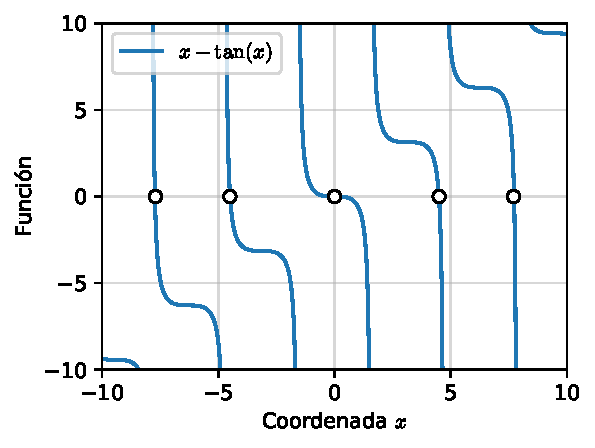
\includegraphics[width=0.65\textwidth]{tan.pdf}
\caption{Función $f(x) = x - \tan x$.}
\label{fig:tan}
\end{figure}

\item \label{ejer:raices-turbo} Se desea determinar el caudal $Q$ con el que es necesario alimentar una turbomáquina que inicialmente está localizada sobre una conducción con una resistencia al flujo ${R_T} = 149$ $\nicefrac{\unit{s}^2}{\unit{m}^5} $, un salto o diferencia de niveles $\Delta H = 500\ \unit{m}$ y una potencia específica $\phi = 2548$ $\nicefrac{\unit{m}^4}{\unit{s}}$. Ajustar los parámetros de manera que el problema tenga solución física.

\item \label{ejer:raices-zapata} En un problema de diseño estructural de cimentaciones se debe determinar la dimensión en planta de una zapata cuadrada de forma tal que no se exceda el esfuerzo admisible sobre la masa de suelo en la cual se va a apoyar. Empleando la teoría de mecánica de sólidos, se puede demostrar que la dimensión de la zapata cuadrada, que no sobrepasa el esfuerzo admisible $(\sigma_\text{adm})$ satisface la siguiente ecuación:

\begin{align}
	H^3 \sigma_\text{adm} - H P \pm 6 (M_1 + M_2) = 0.0
\end{align}

Dónde:

\begin{itemize}
	\item $H:$ Dimensión en planta de la zapata cuadrada.
	\item $\sigma_\text{adm}:$ Esfuerzo admisible.
	\item $P:$ Carga vertical sobre la zapata.
	\item $M_1, \ M_2:$ Momentos flectores al rededor de dos ejes ortogonales.
\end{itemize}

Se desea determinar la dimensión $H$ de la zapata necesaria para no exceder el esfuerzo admisible $\sigma_\text{adm}= 18 \ \unit{tf}/\unit{m}^2$, si la zapata se encuentra sometida a la carga $P=32 \ \unit{tf}$ y los momentos $M_1= 18 \ \unit{tf}\cdot\unit{m}$ y $M_2= 23 \ \unit{tf}\cdot\unit{m}$.

\end{enumerate}